%%
\section{Threat Model of Web Tracking}
\label{sec:threat-model}


%%
Our threat model of web tracking considers four main entities: user, browser, first-party website, and third-parties included in the website. 
%
The user is an individual accessing websites on the Internet through their browser (also known as user agent~\cite{mdnUserAgentMDN2025}), seeking to keep their online behavior private and hence considered the \textit{victim}. % or at least under control. 
%
Browsers mediate all interactions between the user and the web content, enforcing different policies described in~\autoref{sec:background}. % and providing necessary functionality for webpages. 
%
The first-party website is the webpage that the user directly visits to browse content. 
%
It often includes resources from third-parties that are not directly visited by the user and are typically hosted on a different domain than the first-party website~\cite{mdnDomainMDNWeb2024}.
%
A tracker is any party whose goal is to collect data about the user’s activities in order to monitor or identify the user’s behavior across the web. % across one (\textit{same-site tracking}) or more sites (\textit{cross-site tracking}) or across devices (\textit{cross-device tracking}). 
%
We consider first- and third-party trackers as \textit{adversaries}, where their aim is to gather maximal information on users. %consistent with their capabilities.
%
\autoref{fig:threat-model} provides a conceptual overview of our model where \texttt{news.com} and \texttt{sports.com} are the first-party websites visited by the user from their personal device(s). 
%
\texttt{tracker1.com} and \texttt{tracker2.com} are the third-parties embedded in the first-party websites.



\begin{figure}
    \vspace{-2mm}
    \centering
    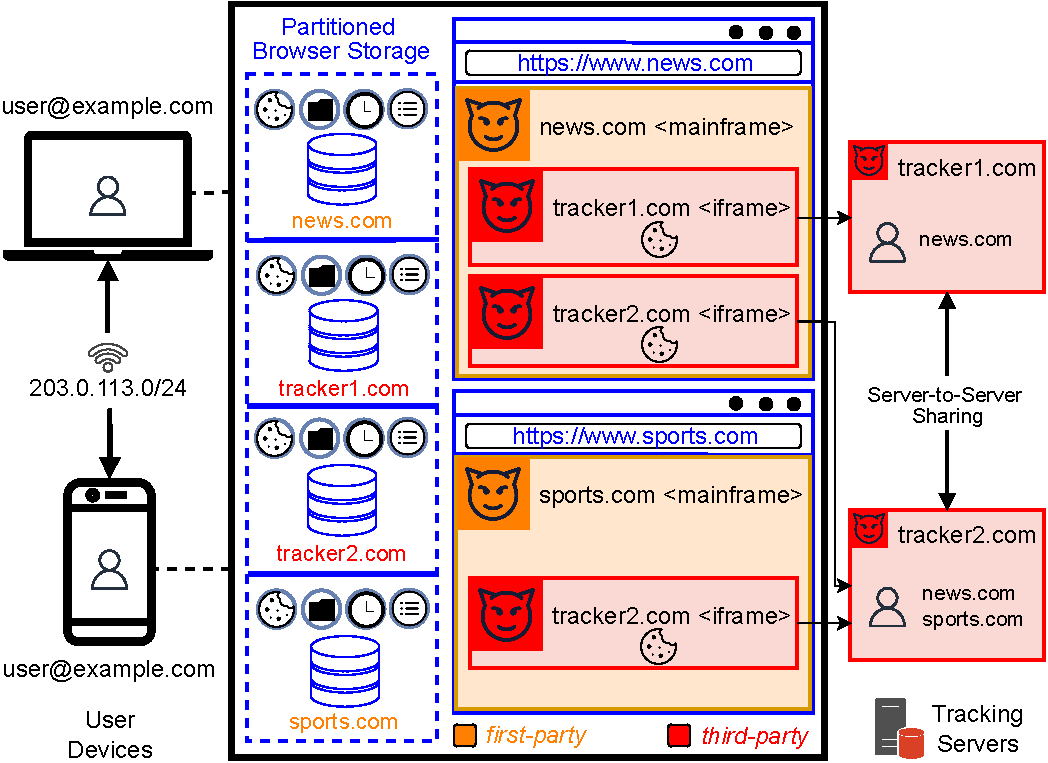
\includegraphics[width=0.99\linewidth]{figures/threat-model.pdf}
    \caption{Threat model of web tracking}
    \label{fig:threat-model}
    % \vspace{-6mm} % submission
    \vspace{-3mm} % arxiv
\end{figure}



%%
\noindent \textbf{Goals of an Adversary.} 
%
% The primary goal of an adversary is to identify and correlate user data across the web for purposes such as profiling, analytics, or ad targeting.
%
User data can be divided into two categories: (1) identifiers such as email or identifying information such as network, software, or hardware configurations, and (2) browsing activity comprising webpages visited and website interactions performed by the user. 
%
The tracker's goal can be distinguished into different scopes:
%
\noindent \textbf{\textit{Same-site}.} 
The tracker aims to monitor or recognize a returning user on the same first-party website across multiple visits or page loads. 
%
\textbf{\textit{Cross-site}.} 
%
Trackers embedded on multiple unrelated first-party websites often aim to uniquely identify and track a user across these sites in order to link different website activities to the same user.
%
\textbf{\textit{Cross-device}.} 
%
A tracker may also aim to identify the same user as they browse the internet using different devices or browsers. 
%
For instance, \texttt{tracker1.com} embedded on \texttt{news.com} would like to know that the user \texttt{X} on a mobile phone is the same as user \texttt{Y} browsing the same website a little later from a desktop device.
%
In summary, the adversary's primary goal is to persistently and uniquely label the user or the user’s browser/device and to collect user data tied to that label, across navigations, sites, and over time, for purposes such as profiling, analytics, or ad targeting.
%
Besides, a secondary goal of the tracker may be to avoid detection or prevention---\ie{}, trackers aim to achieve their goal despite anti-tracking measures.



%%
\noindent \textbf{Capabilities of an Adversary.} 
%
% A tracker's capabilities are shaped by the web's architecture and browser's security model discussed in ~\autoref{sec:background}.
%
To achieve its goals, an adversary's capabilities can be explained in context of \textit{inclusion}, \textit{collection}, \textit{storage}, and \textit{sharing} of the user data, subject to the browser's context-origin restrictions discussed in ~\autoref{sec:background}.
%
The adversary is considered capable enough to track users either in presence of these browser-enforced policy restrictions or by circumventing them.
%
\textbf{\textit{Inclusion}.} 
%
A first-party tracker is assumed to directly monitor user activities within the mainframe context.
%
A third-party tracker could be embedded as an inline resource (\eg{}, image/script tag) within the mainframe context by the first-party assuming trust delegation, an iframe with a separate context under its origin (\ie{}, with its own DOM, state, and resources), or as a resource within a third-party iframe, isolated from the mainframe context. 
%
\textbf{\textit{Collection}.}
%
A tracker aims to collect user data through available browser features by either executing JavaScript code or reading browser storage.
%
By including an executable resource (\eg{}, script) on the webpage, tracker gains the ability to run code in the user’s browser, subject to script execution context requirements governed by browser's context model discussed in Section~\ref{sec:background}.
%
With an embedded non-executable resource (\eg{}, image), a tracker can still initiate resource loading requests to its server, sharing cookies along with the request.
%
We assume the tracker could use one or more inclusion methods described above depending on what the first-party allows.
%
\textbf{\textit{Storage}.}
%
Trackers may read, write, or modify data in the user's browser using \texttt{localStorage}, \texttt{sessionStorage}, \texttt{indexedDB} and the cookie jar.
%
The stored data can be accessed by the tracker in subsequent visits to either the same site or a different site.
%
\textbf{\textit{Sharing}.}
%
Next, the adversary's goal is to share the collected user data with its own servers or a partner's tracking server.
%
For this, trackers can initiate network requests including the user data in one of four ways: (1)~as request URL query parameter, (2) request payload, (3)~request header, or (4) through HTTP cookies.
%
Approaches 1-3 require tracking scripts to explicitly include user data, whereas HTTP cookies associated with the tracker's domain are automatically included in all requests to the tracker's server. % (\eg{}, setting a custom request header for tracking).
%
% In case of 4, browsers automatically attach the previously set tracker's cookies with the requests sent to the tracker’s domain as a request header, even if that request originates in a first-party context. 
%%
We use this threat model to understand different web tracking mechanisms and their evolution over time.